\chapter{Related Work}\label{chapter:Related Work}

\section*{IPv6}

IPv6 was initially released in 1998 \cite{rfc2460}, with the motive of replacing its predecessor IPv4. As per the new specification of IPv6 \cite{rfc8200}, it brings in expanded addressing capabilities,
simpler header format, improved support for extensions and options, flow label capabilities and authentication and privacy capabilities. However, in spite of these upgrades and benefits, IPv6 has not been fully adopted by Internet Service Providers (ISP)
and Content Delivery giants like, Google, Netflix, etc. As per the Google IPv6 adoption statistics \cite{gv6}, IPv6 connectivity at present remains around 24\% worldwide (refer \cref{fig:Google IPv6 Adoption Statistics}. 
Although IPv6 connectivity is low, its increasing exponentially after the \textit{WORLD IPv6 LAUNCH} in June 2012 \cite{ipv6day}. This was an outcome of \textit{WORLD IPv6 DAY} on June 2011, on which major ISPs and content providers decided to enable IPv6, just to test IPv6 performance
and reliability. But, the belief and prediction of having more than 50\% IPv6 user connectivity by 2016 are not achieved \cite{ipv6day}. Sarrar et al. \cite{sarraripv6} reported that although the adoption rate for IPv6 is not what was expected, it's still growing at a
very good rate. The slow adoption rate and because of its importance, IPv6 has been the central focus of several studies, to get a better understanding of the issues that the ISPs are facing.

Colitti et al. from Google \cite{colittiipv6} studied the quality and quantity of IPv6 connectivity in 2010. The main findings of their results reveal that although IPv6 connectivity is growing significantly,
it is not up to the mark. They also said that few larger deployments of IPv6 are influencing the adoption rate and that IPv6 connectivity varies by countries. They also found out that native IPv6 latency is
comparable to IPv4. Dhamdhere et al. in \cite{dhamdhereipv6}, further confirmed the findings of \cite{colittiipv6}. They also found out that IPv6 network deployment is stronger in Europe and Asia, and that Hurricane Electric is the major player in contributing
to the IPv6 network topology. One of the main reason is that Hurricane Electric offers free IPv6 tunneling service to their clients \cite{tunnelbroker}. Wu et al. in \cite{ipv6transition} surveyed
the popular solutions for the transition of IPv4 to IPv6. They reconsider the key problems and issues in IPv4-IPv6 transition and found out that scalability, heterogeneous addressing, and application layer translation are the main issues for the IPv4-IPv6 transition.
Studies by Nikkhah and Guerin \cite{mehdicoordination} \cite{mehdiprogress}, further reports that disagreement among ISPs on migration to IPv6 or offering competing alternatives to IPv6, created a destabilizing effect as they couldn't converge to a common solution.
Also, they reported that little coordination among ISPs in offering IPv6 could go a long way.  Czyz et al. further explores the IPv6 adoption rate in \cite{jakubipv6}, where they are using ten global-scale datasets and considers twelve metrics
and analyzed the IPv6 adoption. According to their results, IPv6 adoption varies by two orders of magnitude depending on the metric being evaluated, and that isolated evaluations must be taken care of. Czyz et al. \cite{jakubipv6} also reported similar to other studies, 
that IPv6 has improved drastically in the past few years and that the IPv6 adoption rate is not globally uniform. Aben in \cite{loststars} reported that despite the improvement of IPv6, many Internet Service Providers disabled IPv6 due to lack of clients interests.
He surveyed the Local Internet Registries which stopped announcing IPv6 and found out that other reasons for disabling IPv6 were the business itself or the network infrastructure changes.

\begin{figure}[!ht]
	\centering
	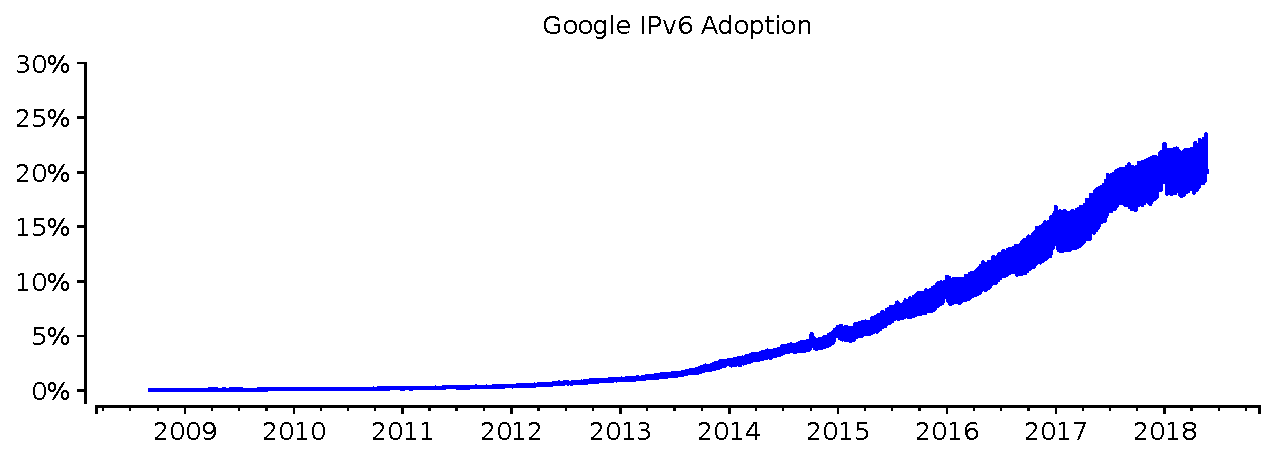
\includegraphics[keepaspectratio, height=5cm, width=15cm]{figures/googlev6stats.pdf}
	\caption[Google IPv6 Adoption Statistics]{Google IPv6 adoption statistics \cite{gv6} for recent years, and its shows that IPv6 adoption has grown exponentially, being around 24\% as of May 2018.}
	\label{fig:Google IPv6 Adoption Statistics}
\end{figure}

\subsection*{Internet Topology}

Dhamdhere et al. in \cite{dhamdhereflat}, reported that the Internet infrastructure and topology is changing and evolving rapidly. They explained that the topology is transitioning from a multi-tier hierarchy of ISPs and transit providers to a horizontal mesh of peering links. Furthermore, Labovitz et al. \cite{topologycraig} explains that the reason for this transition in the Internet topology is the shifting 
of Internet traffic to Content Delivery Networks (mostly video) or consumer networks, which are located within an ISP infrastructure or at Internet Exchange Points (IXPs).
To find out these changes in the Internet topology, many studies used different approaches in the past. Dong et al. \cite{topologydong}, proposed an algorithm which takes
into account multiple protocols, general internet protocols, and routing protocols, and helps discover the network topology. Donnet \cite{topologybenoit} further did a more concrete study on methods of discovering Internet topology, and one of the methods used \textit{traceroute} to study the number of hops in an IP interface. \textit{traceroute} is a very popular
tool used all over the world for network analysis, CAIDA’s Archipelago \cite{caidaark} and RIPE ATLAS \cite{ripeatlas} are such organizations which are using this for large-scale measurements.
\cite{topologybenoit} further explains the limitations of traditional traceroute implementations. It reasons that the same network can result in different network topologies being discovered,
because of routing dependency and load balancing issues of traditional traceroute. Knight et al. \cite{topologysimon}, covered these traceroute issues and asked the ISPs to provide their
network data, which will be made public through Internet Topology Zoo, which is a store of network data consisting of around 200 topologies. Holbert et al. \cite{topologybrett} further
explain that non-cooperative routers towards traceroute can influence the measurements, and as a remedy they developed an algorithm, named iTop, to discover the network topology
when only partial information is available. 

\textit{Paris-Traceroute} proposed by Augustin et al. in \cite{internetbrice}, is one of the improvements over the traditional traceroute, and it ignores incorrect path inferences by forcing the
packets to follow the same route. This variant i.e. \textit{Paris-traceroute} is also used in \texttt{SCAMPER} which is a general purpose and scaling active measurement tool supporting multiple traceroute variants, 
proposed by Luckie et al. \cite{scamper}. Almeida et al. \cite{loadrafael}, implemented and applied the Multipath Detection Algorithm (MDA) which is also used in \textit{paris-traceroute}. They discovered that around
74\% of the IPv6 routes includes one load-balancer. 

\subsection*{Content Caching}

The load-balancers do play an important role in content delivery. As most of the Internet traffic comprises of content delivery (audio and video), content caches and CDNs like \texttt{Akamai}
are necessary to provide Quality of Experience (QoE) to the users. Many studies were done to optimize cache deployments, allocation and throughput problems, and in one such study, Poese
et al. in \cite{cc2} reported that Domain Name System (DNS) controls the major content delivery traffic which leads to ISPs losing control of their content delivery.
Wang et al. further reported in \cite{cc1} that content popularity and network topology plays an important role in content delivery, as optimal cache allocation depends on these factors, even
for content-centric networking. Trade-offs in deploying caches optimally were studied by Hasan et al. \cite{cachehasan}, where they discussed that to provide overlay networks for high cache proximity
and to improve performance, CDNs place their caches within an Autonomous Systems (ASes). Also, the CDNs deploy additional caches to get the desired high performance. Cordero and Bonaventure \cite{cc4}
showed that the path lengths to a more popular content are shorter, which supports the notion of "Internet Flattening". 

Frank et al. \cite{cc3}, discussed that major content providers are doing strategic collaborations with large ISPs to provide better content delivery network solution. They further suggested a system
which can bring content closer to the end-user which will reduce download time, increase capacity and will eventually improve CDN-ISP collaboration. 

\subsection*{Dual-Stack}

In the early 2000s, a prevalent solution for IPv6 adoption was to use dual-stack implementations, i.e. supporting both IPv4 and IPv6 in parallel within the same network infrastructure.
In 2004, Cho et al. \cite{dualcho} reported that the response time of IPv6 connections on dual-stack implementations was bad, due to reasons such as network misconfiguration or other network problems. Pujol et al. \cite{dualpujol}, studied the state of IPv6 traffic share over a dual-stack residential broadband network. They elaborated the difference between
IPv6 "connectivity" and IPv6 "traffic share", explaining that a major fraction of Internet users do have IPv6 connectivity but the IPv6 traffic share is pretty low. As already discussed,
the current rate of IPv6 connectivity is around 24\% as shown in \cref{fig:Google IPv6 Adoption Statistics}, while at Amsterdam Internet Exchange, the IPv6 traffic is around 90Gbps on
an average, whereas the total traffic here around 3.5Tbps, i.e. IPv6 traffic is around 3\% only, as depicted in \cref{fig:AMSIX Statistics}. Pujol et al. reasoned for this discrepancy that home routers were not supporting IPv6, applications were falling back to IPv4, and that service providers were lacking IPv6 support. They further reasoned that the IPv6 network
hierarchy is completely different than IPv4 and that Hurrican Electric has a major role in contributing to IPv6 topology. Also, as the network path from the client to host doesn't completely support IPv6, it affects the fallback behavior. 

As per RFC 6555, which is also referred to as \texttt{Happy Eyeballs} algorithm, IPv6 gets a slight preference over IPv4, and whenever the connectivity is bad, IPv6 can fallback to IPv4.
Bajpai and Schönwälder \cite{bajpaihappy} showed that with a timer value of 300ms, IPv6 connections are preferred 90\% of the time in spite of being slower than IPv4. They further suggested reducing
the timer value to 150ms and discussed that the current value of 300ms is too large as IPv6 performance has improved over the years and thus a reduced value of 150ms will maintain the same preference level for IPv6.
Pujol et al. \cite{dualpujol} also suggested the fallback behavior of IPv6 can be attributed to incompatibility issues rather than IPv6 slowness.

\begin{figure}[!ht]
	\centering
	\begin{minipage}{0.5\linewidth}
		\centering
		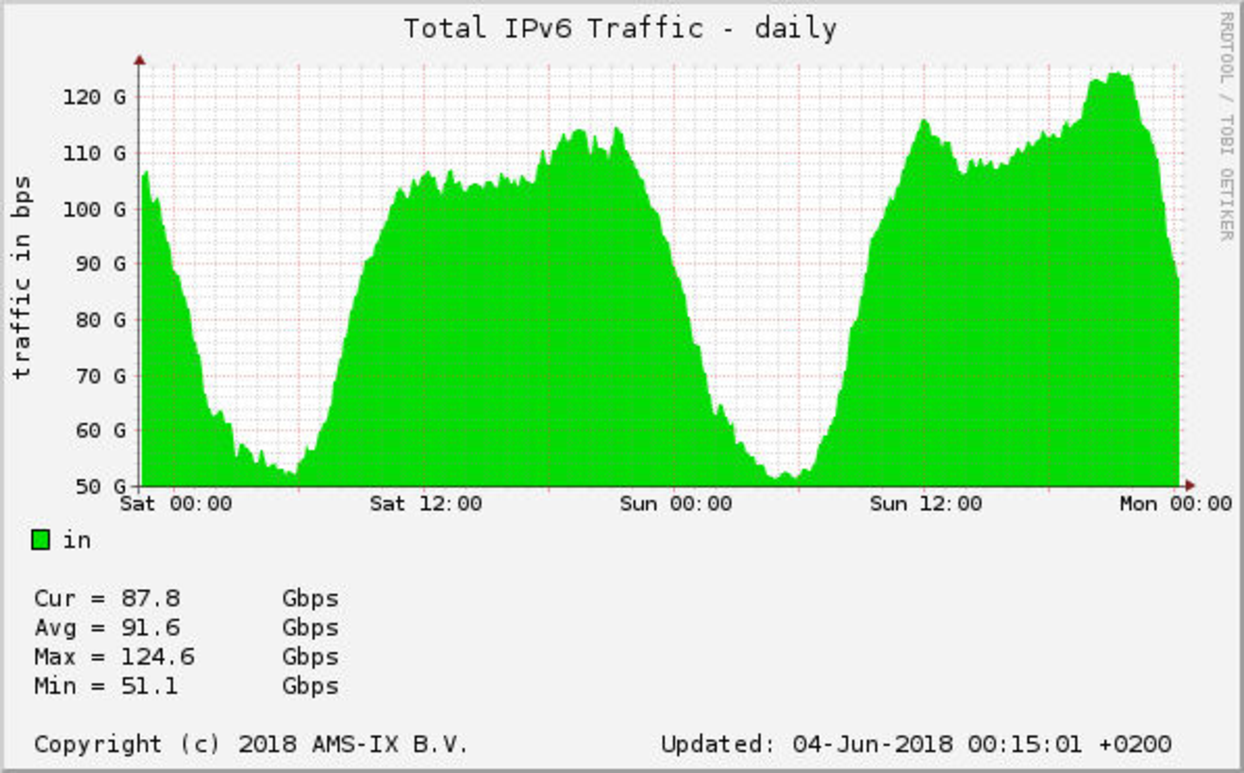
\includegraphics[keepaspectratio, height=5cm, width=12cm]{figures/ipv6daily.pdf}
	%	\caption[IPv6 Stats]{(a)}
	\end{minipage}
	\begin{minipage}{0.5\linewidth}
		\centering
		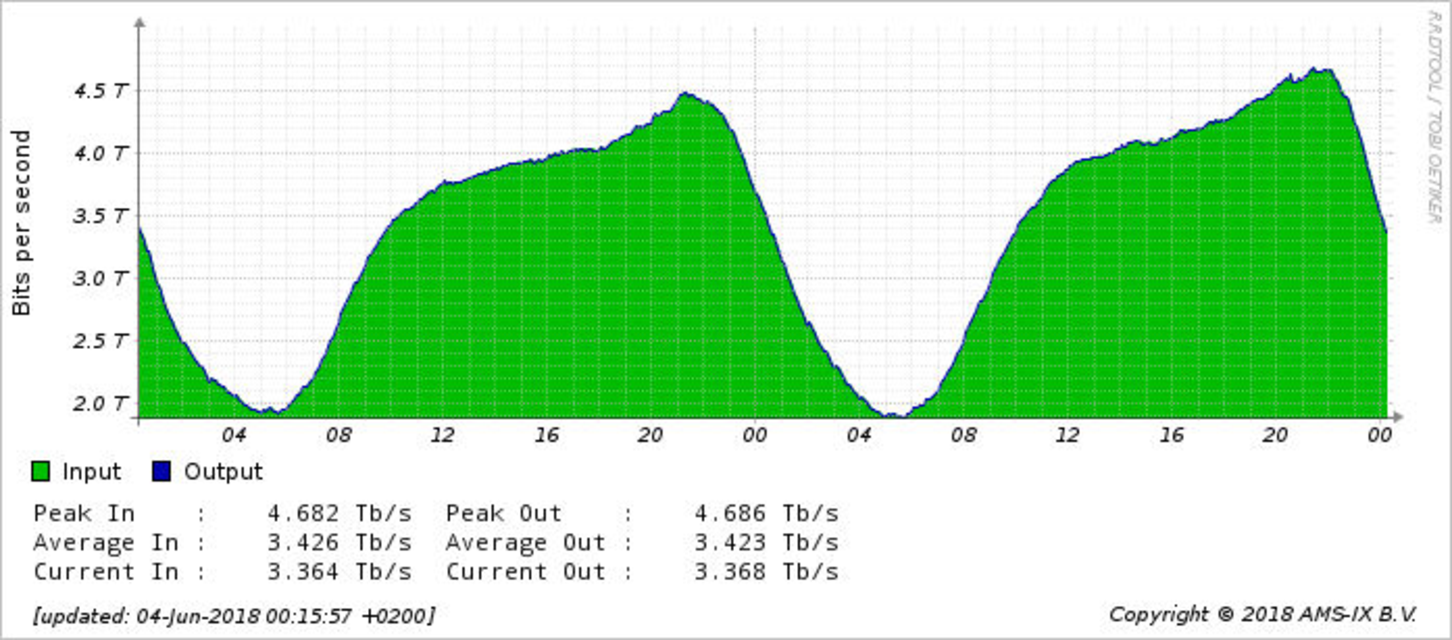
\includegraphics[keepaspectratio, height=5cm, width=8cm]{figures/totalstats.pdf}
		%\caption[Total Stats]{(b)}
	\end{minipage}
	\caption[AMSIX Statistics]{Internet traffic at Amsterdam Internet Exchange on 4th June 2018, showing IPv6 traffic \cite{ipv6ams} and total traffic \cite{statsams}. 
	As per the graphs, IPv6 traffic accounts to around 3\% of the total traffic on average.}
	\label{fig:AMSIX Statistics}
\end{figure}

\subsection*{IPv4 versus IPv6}

The dual-stack implementation discussed above, enable comparison of IPv4 and IPv6, and in a study by Zhou et al. \cite{46zhou}, analyzed and compared the end-to-end delay and hop count of IPv6 
and IPv4. They published that bad configuration could be a reason for IPv6 to show larger delay times as compared to IPv4. Berger et al. in \cite{46caida} further compare the latency
and loss from Akamai networks over both IP versions. They established that tunneled services showed higher latency and loss depending on the geographical and topological locations.
Wu and Zhou \cite{46wu} evaluated the throughput over IPv4 and IPv6 and established that throughput over IPv6 is slightly higher than IPv4. Nikkhah et al. \cite{ipv6mehdi}, monitored a list of websites from ALEXA's top 1 Million ranking and argued that the data planes for both address families performed comparatively and that routing is the reason for poor performance over IPv6. Li et al. \cite{46li} further establish
that actual traffic features such as packet sizes, packet flows and traffic volume are quite different among both address families.

The previous studies discussed showed that IPv6 performed poorly as compared to IPv4, but recent studies indicate that IPv6 performance is improving with time. 
Giotsas et al. \cite{46giotsas} studied the convergence of IPv4 and IPv6 topologies and found out that relationship between IPv6 ASes is forming the same trend as IPv4 and the routing paths are also becoming similar. They also pointed out that Hurricane Electric influenced these results. Bajpai and Schönwälder \cite{46bajpai} further compared the IPv4 and IPv6 TCP connect times towards dual-stacked websites and found out,
that the performance was comparable but the difference could be attributed to the presence of content caches in ISP for IPv4 which improves the connect times for IPv4. Hyun et al. \cite{46hyun} further did a similar analysis
for the mobile networks and reported that around 85\% of the dual-stacked websites experienced better TCP connect times over IPv4 as compared to IPv6 and reasoned that this is due to lack of IPv6
infrastructure in the mobile network.

Livadariu et al. \cite{46liva}, measured the routing dynamics in the control plane of IPv4 and IPv6 and found out that IPv4 is more stable here, whereas for the data plane both address
families show comparable performance. They attributed that network congestion leads to low performance, as IPv4 and IPv6 share the same infrastructure as well.

\subsection*{IPv6 Address Space}
Understanding the network topology is very important to figure out the growth of the Internet. Lutu et al. \cite{addresslutu} and Beverly et al. \cite{addressbeverly} did a study to
understand the reachability of prefixes and availability of routers for IPv6. Similarly, Li et al. \cite{addressli} found out that even though when the traffic is skewed, around 60\% of the IPv6 prefixes are reachable from multiple paths. Beverly and Berger \cite{beverly2} developed an active measurement technique to find out "server siblings" i.e. both IPv4 and IPv6 addresses corrosponds to one physical machine. They further established that understanding the sibling and non-sibling relation gives insight about the co-relations, enhance IPv6 geolocation lookups, and helps compare paths.

\section*{Netflix}

Netflix has become an Internet giant in providing content and generating Internet traffic all over the world (around 190 countries), it is reportedly having around 109 million customer base \cite{ninanetflix}. In 2015, The Washington Post published an article \cite{washingtonnetflix} stating that Netflix accounts for 37\% of Internet downstream traffic in North America. Given the immense growth of Netflix as a 
content provider, few studies have analyzed Netflix Open Connect Appliance (OCA) architecture, its traffic, and its caching architecture. 
Adhikari et al. \cite{adhikarinetflix} published their study in early 2012, where they focused on Netflix architecture and its service strategy. As per their findings, 
Netflix uses a blend of cloud services such as Amazon AWS, CDNs, other public services and little infrastructure of their own for the content delivery. They also propose their strategy to improve video content delivery using multiple CDNs, which is choosing the best performing CDN based on a small measurement conducted in the beginning of the video playback claims to improve 12\% bandwidth over a single CDN, 
and more than 50\% improvement in case of using multiple CDNs. In 2013, Martin et al. presented a study \cite{martinnetflix}, where they considered Netflix as a Dynamic Adaptive Streaming over HTTP (DASH) application and characterized
the bandwidth consumption of Netflix. They further suggested that during stable network congestion, Netflix adaptation defaults to the TCP control, whereas in case of unstable network congestion, the algorithm is twisted with TCP control.
Adhikari et al. further did a study on the Netflix and Hulu CDNs in \cite{adhikarihulu}, here they reveal that both Netflix and Hulu are heavily using third-party infrastructures such as Amazon AWS or Akamai. Both the platforms consider the
video request to select the CDN, without considering the network conditions. Furthermore, the available bandwidth for Netflix and Hulu CDN varies according to the geographical regions.
Adhikari et al. measured the available bandwidth by conducting light-weighted measurements at the beginning of the playback and found the similar results they published in \cite{adhikarinetflix} in 2012, i.e. 
an improvement of 12\% bandwidth when a single CDN is used and more than 50\% improvement in bandwidth when using multiple CDNs. 
Netflix in 2012 started its own CDN named "OpenConnect" \cite{netflixoca} and a recent study conducted by B{\"o}ttger and et al. 
discussed the Open Connect Appliances (OCAs) in \cite{openconnect}, where they studied the infrastructure deployment of Netflix and how Netflix is using 
Internet Exchange Points(IXPs) to deliver its video content all over the world. The authors described how Netflix OCAs help to peer with ISPs for free because of these IXPs, saving transit and content delivery costs. 
Furthermore, they showed in \cite{openconnect} that Netflix is present in nine of the top ten largest IXPs of the world, Netflix infrastructure presence in major parts of the world (signifying global presence), and their analysis about the internet traffic generated by Netflix is consistent over different geographical regions. B{\"o}ttger et al. further claims that all these factors make Netflix a hypergiant as a content distribution provider.
 

\subsection*{Netflix OCA Architecture}

\begin{figure}[!ht]
	\centering
	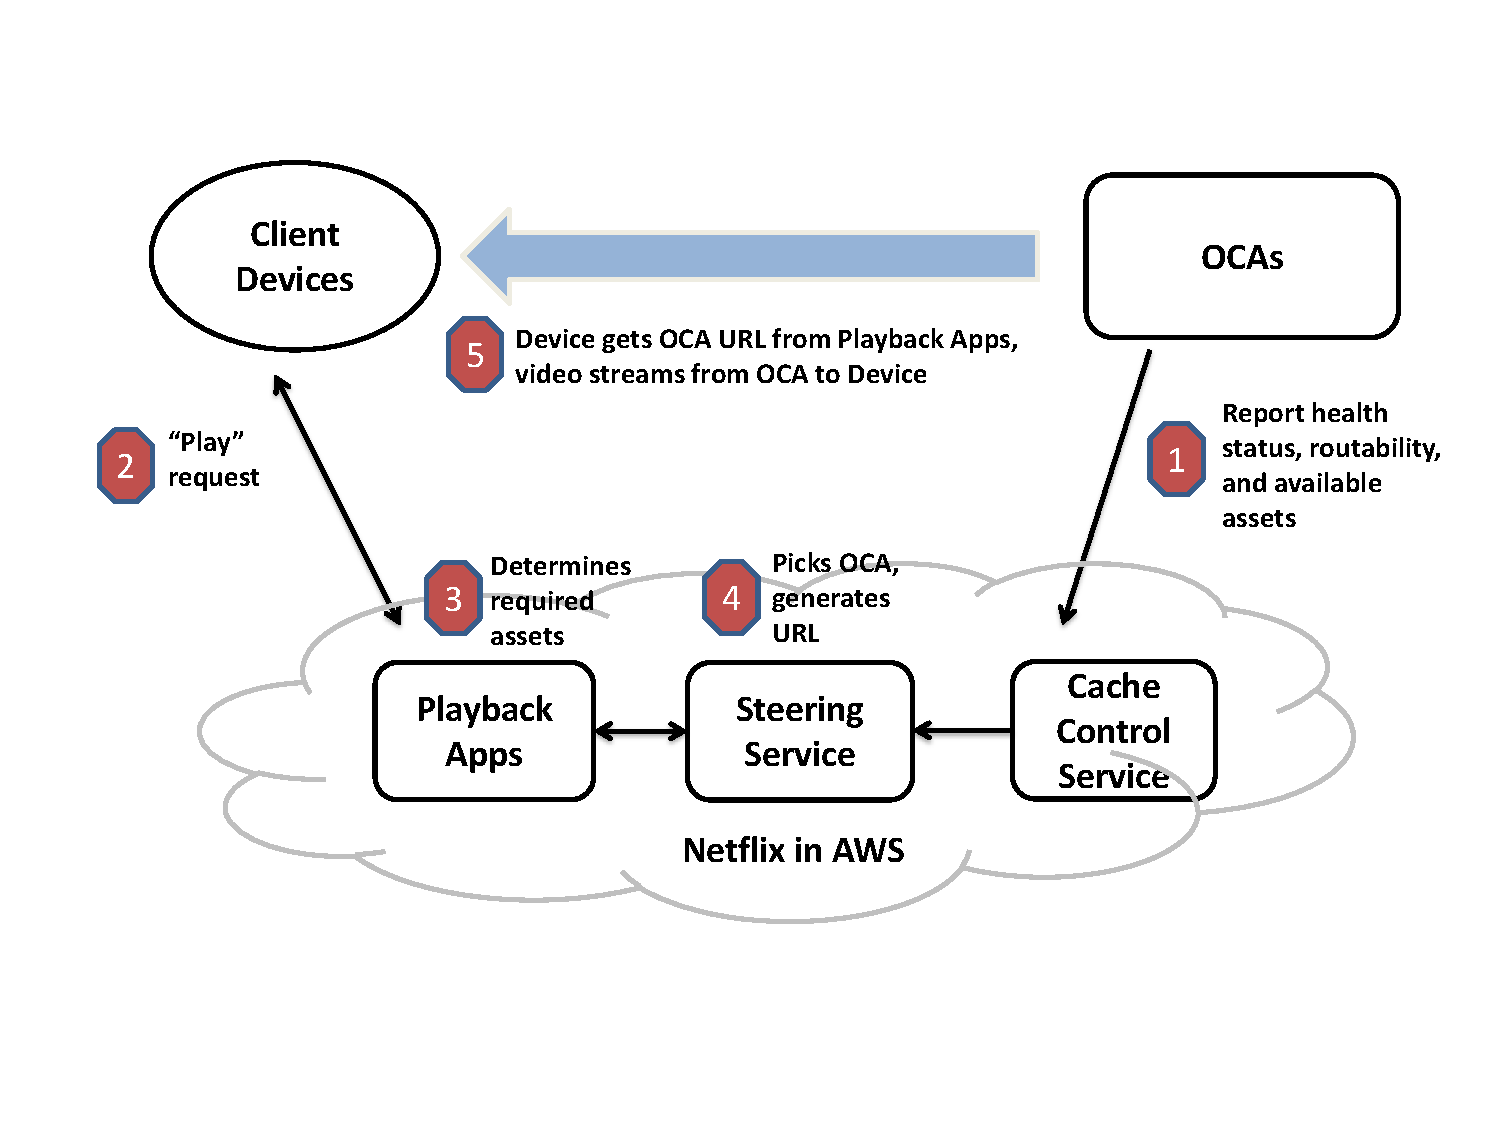
\includegraphics[keepaspectratio, height=8cm, width=15cm]{figures/netflix-oca-architecture.pdf}
	\caption[Netflix OCA Architecture]{Netflix playback process depicting the process of OCA selection and Content Delivery to the customers (figure referred from \cite{ocaoverview}). Variables that define the particular OCA selection is based on location or 
	load on the server, number of TCP connections, and content distribution \cite{netflixfast}.}
	\label{fig:Netflix OCA Architecture}
\end{figure}

The working of Netflix Open Connect CDN infrastructure \cite{ocaoverview} is the foundation of the \texttt{netflix} test (explained in chapter \ref{chapter:Datasets}) that we are using to get the data. 
The building blocks of the Open Connect CDN is the Open Connect Appliance (OCA) which are purpose-built server hardware appliances and store the Netflix video content \cite{ocaoverview}. These OCAs doesn't store client data and are installed at Internet Exchange Points (IXPs) or within the ISPs. 

As depicted in \cref{fig:Netflix OCA Architecture}, the clients or end users interact with the Netflix application which acts as a control plane and is hosted on Amazon AWS.
The OCAs also communicate health and routability to this control plane. When the Netflix application verifies the user authorization, the control plane determines the characteristics such as user location, network conditions, server utilization and content distribution to select the OCAs which will be used to stream the content to the user. The Netflix control plane generates URLs for these OCAs and 
deliver it to the client, and then the client redirects to these OCAs and the video streaming starts.